\documentclass[]{report}

% All Dependencies

\usepackage{graphicx}
\usepackage{float}
\usepackage{amsmath}


% Title Page
\title{MATH 4820 - Homework 1}
\author{Jack Reilly Goldrick}


\begin{document}
\maketitle


\section{Problem 1}

\subsection{Exercise 1.4.2}
%																					IMAGE 																												  %
%%%%%%%%%%%%%%%%%%%%%%%%%%%%%%%%%%%%%%%%%%%%%%%%%%%%%%%%%%%
\begin{center}
	

	\begin{figure}[H]
		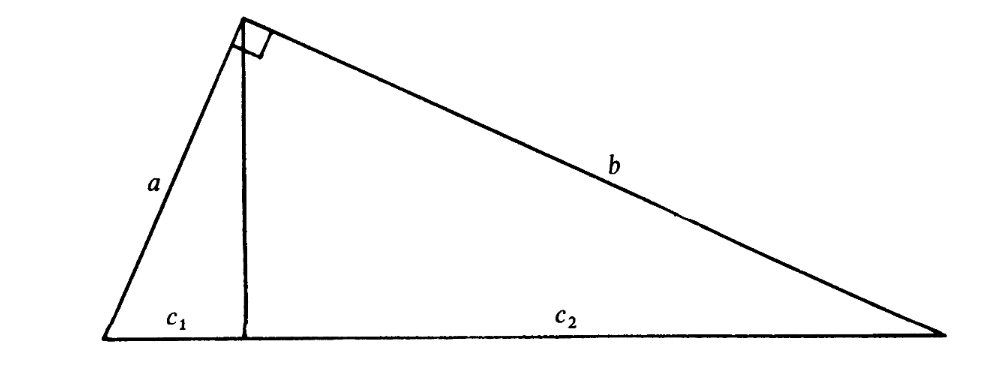
\includegraphics[width=10cm] {pics/1-triangle}
		
	\end{figure}
	
\end{center}
%%%%%%%%%%%%%%%%%%%%%%%%%%%%%%%%%%%%%%%%%%%%%%%%%%%%%%%%%%%




%																					PROOF  	    									     															     %
%%%%%%%%%%%%%%%%%%%%%%%%%%%%%%%%%%%%%%%%%%%%%%%%%%%%%%%%%%%
\subsubsection{Proof}

\begin{itemize}
	\item Let $ c =  c_1 + c_2 $, $h$ denote the vertical segment, and A, B, C, H denote the vertexes across from a respective segment such that C is the vertex that connects $a \land b$,  A connects $c_{2}$ to $b$ and H connects $c_1$  and $c_2$ to $h$.
	
	\item Let $\triangle ABC , \triangle ACH, and \triangle BCH$ all be right triangles since they all have one right angle  
	
	\item $\triangle ABC $ shares a unique vertex, thus angle, other than the right angle, $\angle CAB$  with $\triangle ACH$ and a separate unique angle that is not right, $\angle CBA$, with $\triangle  BCH$
	
	\begin{itemize}
		\item The larger triangle ABC has two  angles that are equal to either two of the smaller triangles' angles.  Thus given the properties of a triangle, the third angle must be equal to either of the larger triangle's remaining angle with respect to the smaller subdivision, meaning that all triangles are composed of the same combination  of angles.
		\begin{itemize}
			\item Thus all three triangles are similar.
		\end{itemize}
	\end{itemize}
	
	\item  Given that all the triangles are similar the following equations hold true:
					\begin{center}
						
						\begin{equation}
							\frac{a}{c_{1}} = \frac{ c_{1} + c_{2}}{a} 
						\end{equation}  
					
						\begin{equation}
							 \frac{b}{c_{2}} = \frac{ c_{1} + c_{2}}{a} 
						\end{equation}
						
					\end{center}
					
	\item Cross-multiplying the equations we have:
					\begin{center}
						
						\begin{equation}
							a^{2}= ( c_{1} + c_{2}) (c_1) =  c * c_1
						\end{equation}  
						
						\begin{equation}
							b^{2}= ( c_{1} + c_{2}) (c_2) = c * c_2
						\end{equation}
						
					\end{center}
					
	\item Adding equations (3) and (4) we have:
					\begin{center}
	
						\begin{equation}
							a^{2} + b^{2}= c * c_1 + c * c_2 
						\end{equation}  
						
						
					\end{center}				
					
					
					
	\item Rearranging Equation (5) we have:
				\begin{center}
					\begin{align*}
						a^{2} + b^{2} &= c * c_{1} + c * c_{2}  \\
												   &= c *(c_1 + c_2 ) \\
												   &=  c * c \\ 
												   &= c^{2}
					\end{align*}
					
					
				\end{center}
	\item Since $ 	a^{2} + b^{2} = c^{2}$ for right triangle ABC, we have proven the Pythagorean Theorem.
\end{itemize}


\section{Problem 2}

\subsection{Infinitely Many Triples}


Since we know from the parameterization of triples in class that all we need is a pair of numbers (m, n)  that are coprime with opposite parity.  Since there are infinitely many co-prime integer pairs with opposite parity, we can conclude that there exists infinitely many triples since infinitely many primitive triples exist.


\section{Problem 3}

\subsection{Finitely many Triples for a=100}
	\begin{itemize}


	\item Constructing the Theorem from the variables we have:
		\begin{center}
	
		\begin{equation}
			a^{2} + b^{2} = c^2 = 10^4 + b^{2} 
		\end{equation}  
	
		\begin{equation}
			c^{2} - b^{2} = 10^{4}
		\end{equation}
	
	\item  From equation (7) we have:				
			\begin{align*}
				c^{2} - b^{2}& = 10^{4}  \\
				(c - b) * (b + c)&= (2^4) * (5^4)
			\end{align*}
				
			\end{center}
	\item Thus from the prime factorization formula, we know $a^2$, in this case, has 25 factors resulting in 12 pairs of factors.
	
	\item Let $ x =  c - b \land y = c + b$ 
	
	\item rearranging we have $ c = x + b \land b = y - c$. This results in the following two equations:
		\begin{center}
	
			\begin{equation}
			c= \frac{x + y}{2}
			\end{equation}  
	
			\begin{equation}
				b=\frac{y - x}{2}
			\end{equation}
	
	
		\end{center}	
		
		
			\item Since this construction does not generate only primitive triples since b is always even, and $a^2$ has finitely many factor pairs, we can conclude that there are only finitely many triples for $a=100$
	\end{itemize}
	

\end{document}          
